% !TeX program = lualatex
% !TeX encoding = utf8
% !TeX spellcheck = uk_UA
% !TeX root =../LabWork.tex

\part{Інтерференція світла}

\nocite{akhmanov, Godzhaev}
\printbibliography[title={Рекомендована література}, heading=subbibliography]

\section{Означення}

Під інтерференцією світла розуміють явища, в яких при накладенні двох або більше світлових хвиль відбувається просторовий перерозподіл їх енергії, при цьому виникають стійкі в часі світлі і темні ділянки, що чергуються в просторі --- так звані інтерференційні смуги. 

Нехай в деяку точку приходять дві гармонійні хвилі, напруженості поля яких змінюються згідно із законами:

\begin{equation}\label{eq:EField}
    \vect{E}_1 = \vect{E}_{01}\cos\omega_1 t, \quad \vect{E}_2 = \vect{E}_{02}\cos(\omega_2 t + \phi).
\end{equation}

Відповідно до принципу суперпозиції напруженість результуючої хвилі дорівнює сумі напруженостей вихідних хвиль:

\begin{equation*}
    \vect{E} = \vect{E}_1 + \vect{E}_2,
\end{equation*}

А інтенсивність результуючої хвилі  пропорційна усередненому за часом квадрату напруженості:
\begin{equation}\label{eq:Intens}
    I \sim \left\langle\left(  \vect{E}_1 + \vect{E}_2\right)^2  \right\rangle  = \left\langle E_1^2\right\rangle + \left\langle E_2^2\right\rangle  + 2\left\langle \vect{E}_1 \cdot \vect{E}_2 \right\rangle.
\end{equation}

Доданок $\left\langle \vect{E}_1 \cdot \vect{E}_2 \right\rangle$ називається \emph{інтерференційним}, оскільки саме він відповідальний за існування інтерференційної картини. Цей доданок дорівнює нулю в наступних випадках:
\begin{enumerate}
    \item напрямки коливань векторів $\vect{E}_1 $ та $\vect{E}_2 $ є взаєоперпендмкулярними;
    \item частоти коливань $\omega_1$ та  $\omega_2$ є різними;
    \item різниця фаз хвиль $\phi$ в будь-якій точці простору змінюється дуже швидко (в  порівнянні з часом спостереження) і хаотично.
\end{enumerate}

Отже, для спостереження інтерференційної картини необхідно, щоб всі попередні умови не виконувались.

Розглянемо дві хвилі, які поляризовані в однієї площині, мають однакову частоту і сталу різницю фаз:
\begin{equation}\label{eq:CogEField}
    \vect{E}_1 = \vect{E}_{01}\cos\omega t, \quad \vect{E}_2 = \vect{E}_{02}\cos(\omega t + \phi), \quad \vect{E}_{01} \parallel \vect{E}_{02}.
\end{equation}
такі хвилі називаються \emph{когерентними}. Підставляючи ці вирази в формулу~\eqref{eq:Intens}, знайдемо, що результуюча інтенсивність таких хвиль дорівнюватиме:
\begin{equation}\label{key}
    I = I_1 + I_2 + 2\sqrt{I_1I_2}\cos\phi.
\end{equation}

Крім того, якщо інтенсивності хвиль в певній точці простору однакові $I_1 = I_2 = I_0$, то результуюча інтенсивність дорівнюватиме:
\begin{equation}
    I = 2I_0\left(1+ \cos\phi \right) .
\end{equation}
Отже, як видно з останньої формули, умовою того, що в даній точці буде спостерігатись максимум чи мінімум інтерференційної картини залежить від різниці фаз $\phi$ між хвилями, а саме:
\begin{equation}\label{eq:InterferenceCondition}
    \phi=
    \begin{cases}
        2 m \pi, &\quad \text{умова максимуму інтерференції}, \\
        \left( 2m + 1 \right) \pi , &\quad\text{умова мінімуму інтерференції},
    \end{cases}
\end{equation}
де $m \in \mathbb{Z}$.

\section{Різниця ходу хвиль}

Рівняння гармонічної хвилі має вигляд:
\[
    \vect{E} = \vect{E}_{0}\cos(k r - \omega t),
\]
де аргумент косинуса $ k r - \omega t $,= називається фазою хвилі, а $k = \frac{2\pi}{\lambda}$~--- хвильове число.  Якщо дві монохроматичні хвилі приходять в одну точку простору, то цій точці різниця фаз між хвилями визначається за формулою:
\[
    \phi = ( k_2 r_2 - \omega t) - ( k_1 r_1 - \omega t) = k_2 r_2 - k_1 r_1.
\]

Хвилі можуть поширюватись в різних середовищах з різними показниками заломлення. Хоча хвилі мають однакову частоту, але в середовищах з різним показником заломлення вони мають різну довжину хвилі, яка в $n$ разів ($n$ абсолютний показник заломлення) менша ніж у вакуумі $\lambda = \frac{\lambda_0}{n}$, а тому, хвильове число також буде різним. В оптиці прийнято використовувати саме довжину хвилі світла в вакуумі, а тому різниця фаз буде визначатись як:
\[
    \phi  = k_2 r_2 - k_1 r_1 = \frac{2\pi}{\lambda_0} (n_2 r_2 - n_1 r_1).
\]
Величина 
\begin{equation}\label{eq:optdeiff}
    \Delta = n_2 r_2 - n_1 r_1
\end{equation}
називається оптичною різницею ходу хвиль, натомість величина $r_2 - r_1$ називається геометричною різницею ходу. Не важко зрозуміти, що у вакуумі ці величини співпадають. Крім цього, умови максимуму та мінімуму інтерференції~\eqref{eq:InterferenceCondition} можна переписати для оптичної різниці ходу:
\begin{equation}\label{eq:InterferenceConditionDelta}
    \Delta=
    \begin{cases}
        m \lambda, &\quad \text{умова максимуму інтерференції}, \\
        (2m + 1)\frac{\lambda}{2}, &\quad\text{умова мінімуму інтерференції},
    \end{cases}
\end{equation}
де $m \in \mathbb{Z}$, $\lambda = \frac{\nu}{c}$~--- довжина хвилі світла у вакуумі (індекс <<0>> для зручності не вказаний).

\section{Ітерференційні схеми}

Нехай у нас в розпорядженні є два точкових монохроматичних джерела (довжина хвилі $\lambda$, інтенсивність кожного $I_0$ і розташовані вони на відстані $d$ один від одного. Знайдемо, як буде виглядати інтерференційна картина на екрані віддаленому від джерел на відстань $L \gg d$.

\subsection{Схема Юнга}

Площина екрану паралельна до лінії $\overline{S_1S_2}$, що з'єднує два джерела (рис.~\ref{fig:YoungScheme}). Дане розташування прийнято називати \emph{схемою Юнга}. Знайдемо різницю ходу $\Delta = r_2 - r_1$ між променями, що йдуть від джерел $S_1$ і $S_2$ в точку $P$ з координатою $y$. Початок координат помістимо в точці $O$, відносно якої джерела світла $S_1$ і $S_2$ розташовані симетрично.

\begin{figure}[!h]
	\centering
	\begin{tikzpicture}
		\coordinate (Q) at (0,3.5);
		\coordinate (O1) at (0.25,3.5);
%		\foreach \i in {1,...,3} {\fill[cyan, draw=black] (0,{5/2*(\i-1)}) coordinate (LC\i) rectangle +(0.25,2);}
%		\foreach \i in {0,...,2} {\draw[thick, green!70!blue] (-2-0.5*\i,0) -- +(0,7);}
%		\foreach \i in {0,...,6} {\draw[-latex, orange!80!black] (-3.1,{\i + 0.5}) -- +(1.15,0);}
		\draw[thick] (8,-1) -- coordinate (O) coordinate[pos=0.945] (P) +(0,9); % Ecran
		\fill (P) circle(0.05) node[above left] {$P$};
		\draw (Q) -- (O) node [below left] {$O$};
		\draw[dashed]  (O1) -- (P);
		\draw ([xshift=1.5cm]O1)  let \p{PO1}=( $(P) - (O1)$) in arc (0:atan(\y{PO1}/\x{PO1}):1.5) node[pos=0.5, right] {$\theta$};
		\draw[red!80!black, decoration={
					markings,
					mark=at position 0.5 with {\arrow{latex}}}, postaction={decorate}] (0.25, 2.25 + 2.5) coordinate (S2R) -- node[above, black] {$r_{2}$}(P);
        \fill[red] (S2R) circle(0.1);
		\draw[red!80!black, decoration={
					markings,
					mark=at position 0.5 with {\arrow{latex}}}, postaction={decorate}] (0.25, 2.25 ) coordinate (S1R) -- node[below right, black] {$r_{1}$}  (P);
        \fill[red] (S1R) circle(0.1);
        \draw (S2R) -- (S2R|- 8,-1);
		\draw [dashed] (S2R) -- ($(S1R)!(S2R)!(P)$) coordinate (RA);
		\draw ([yshift=-0.7cm]S2R) let \p{PR}=( $(S2R) - (RA)$) in arc (-90:{atan(\y{PR}/\x{PR})}:0.7) coordinate[pos=0.5] (TH);
		\draw (TH) -- +(60:2) node[above] {$\theta$};
		\draw[decorate,decoration={brace,amplitude=5pt,mirror, raise=0.5ex}] (S1R) -- node[below right=0.5ex] {$\Delta$} (RA);
		\begin{scope}[on background layer]
			\fill[cyan!10] (O1) -- (P) -- (O) -- cycle;
			\fill[yellow!10] (S2R) -- ($(S1R)!(S2R)!(P)$) -- (S1R);
		\end{scope}
		\draw ([xshift=-0.1cm]S2R)  -- coordinate[pos = 0.8] (d2) ([xshift=-1.5cm]S2R) ;
		\draw ([xshift=-0.1cm]S1R)  -- coordinate[pos = 0.8] (d1) ([xshift=-1.5cm]S1R) ;
		\draw (d2) -- node[fill=white] {$d$} (d1);

		\draw ([xshift=0.1cm]P)  -- coordinate[pos = 0.8] (y1) ([xshift=1cm]P) ;
		\draw ([xshift=0.1cm]O)  -- coordinate[pos = 0.8] (y0) ([xshift=1cm]O) ;
		\draw (y1) -- node[fill=white] {$y$} (y0);
		\node at ([shift={(-0.5,0.3)}]S2R) {$S_2$};
		\node at ([shift={(-0.5,-0.3)}]S1R) {$S_1$};

		\draw[latex-latex] (0.25,0.5) -- node[fill=white] {$L$}({P|-0.5,0.5});

		\foreach \i in {-8,...,8} { \path[bottom color=white,  top color=white, middle color = red] (9,{0.5*\i+3.25}) rectangle +(1,0.5); }
	\end{tikzpicture}
	\caption{Схема Юнга}
	\label{fig:YoungScheme}
\end{figure}

Із геометрії рисунка
\begin{align*}
	r_1^2 = {r^2} + {\left( y - \frac{d}{2}\right) ^2}, \\
	r_2^2 = {r^2} + {\left( y + \frac{d}{2}\right) ^2}.
\end{align*}

Звідки випливає, що
\begin{equation*}
	r_2^2 - r_1^2 = 2yd,
\end{equation*}
або
\begin{equation*}
	({r_2} + {r_1})({r_2} - {r_1}) = 2yd.
\end{equation*}

 Відстань $y$, в межах якого утворюються інтерференційні смуги, також значно менше $L$. За цих умова можна вважати, що 
\[{r_2} + {r_1} \cong 2L.\] 

Тоді \[{r_2} - {r_1} = \frac{{yd}}{L}.\] В середовищі з показником заломлення $n \approx 1$ різниця дає оптичну різницю ходу $\Delta$ . Отже, можна написати:
\begin{equation}
	\Delta  = \frac{{yd}}{L}.
\end{equation}

Різниця фаз хвиль $\phi$, яка визначається як:
\begin{equation}\label{eq:Phase_Diff}
    \phi = \frac{2\pi}{\lambda} \Delta
\end{equation}
у випадку схеми Юнга дорівнює:
\[
    \phi = \frac{2\pi}{\lambda} \frac{{yd}}{L}.
\]

Використовуючи умову максимуму інтерференції (для різниці ходу $\Delta = m\lambda$), отримаємо положення самих цих максимумів:
\begin{equation}
	y_{\max} = \frac{{mL}}{d}\lambda.
\end{equation}

Відстань між двома сусідніми максимумами інтенсивності називається відстанню між інтерференційними смугами.  З останнього виразу випливає, що відстань між сусідніми максимумами матиме значення:
\begin{equation}\label{eq:widthofmax}
	\Delta y = \frac{L}{d}\lambda.
\end{equation}

\subsection{Інтерференційні кільця}

Площина екрану перпендикулярна до лінії $\overline{S_1S_2}$, що з'єднує два джерела (рис.~\ref{fig:Rings}). Знову ж знайдемо різницю ходу $\Delta = r_2 - r_1$ між променями, що йдуть від джерел $S_1$ і $S_2$ в точку $P$ з координатою $y$.

\begin{figure}[!h]
	\centering
	\begin{tikzpicture}
		\coordinate (Q) at (0,3.5);
		\coordinate (O1) at (0.25,3.5);
%		\foreach \i in {1,...,3} {\fill[cyan, draw=black] (0,{5/2*(\i-1)}) coordinate (LC\i) rectangle +(0.25,2);}
%		\foreach \i in {0,...,2} {\draw[thick, green!70!blue] (-2-0.5*\i,0) -- +(0,7);}
%		\foreach \i in {0,...,6} {\draw[-latex, orange!80!black] (-3.1,{\i + 0.5}) -- +(1.15,0);}
		\draw[thick] (8,-1) -- coordinate (O) coordinate[pos=0.945] (P) +(0,9); % Ecran
		\fill (P) circle(0.05) node[above left] {$P$};
		\draw (Q) -- (O) node [below left] {$O$};
%		\draw[dashed]  (O1) -- (P);
%		\draw ([xshift=1.5cm]O1)  let \p{PO1}=( $(P) - (O1)$) in arc (0:atan(\y{PO1}/\x{PO1}):1.5) node[pos=0.5, right] {$\theta$};
		\draw[red!80!black, decoration={
					markings,
					mark=at position 0.5 with {\arrow{latex}}}, postaction={decorate}] (0.25, 3.5) coordinate (S2R) -- node[above, black] {$r_{2}$}(P);
        \fill[red] (S2R) circle(0.1);
		\draw[red!80!black, decoration={
					markings,
					mark=at position 0.5 with {\arrow{latex}}}, postaction={decorate}] (2.25, 3.5 ) coordinate (S1R) -- node[below right, black] {$r_{1}$}  (P);
        \fill[red] (S1R) circle(0.1);
        \draw (S2R) -- (S2R|- 8,-1);
%		\draw [dashed] (S2R) -- ($(S1R)!(S2R)!(P)$) coordinate (RA);
		\draw ([xshift=0.7cm]S2R) let \p{PR}=( $(S2R) - (P)$) in arc (0:{atan(\y{PR}/\x{PR})}:0.7) node[anchor = west, pos=0.7] {$\theta$};

		\draw ([xshift=0.7cm]S1R) let \p{PR}=( $(S1R) - (P)$) in arc (0:{atan(\y{PR}/\x{PR})}:0.7) node[anchor = west, pos=0.7] {$\theta$};

		\draw[decorate,decoration={brace,amplitude=5pt, raise=0.5ex}] (S2R) -- node[pos=0.5, above=1ex] {$\Delta$} ($(S2R)!(S1R)!(P)$);

		\draw (S1R) -- ($(S2R)!(S1R)!(P)$);

		\draw ([yshift=-0.1cm]S2R)  -- coordinate[pos = 0.8] (d2) ([yshift=-1.5cm]S2R) ;
		\draw ([yshift=-0.1cm]S1R)  -- coordinate[pos = 0.8] (d1) ([yshift=-1.5cm]S1R) ;
		\draw[latex-latex] (d2) -- node[fill=white] {$d$} (d1);

		\draw ([xshift=0.1cm]P)  -- coordinate[pos = 0.8] (y1) ([xshift=1cm]P) ;
		\draw ([xshift=0.1cm]O)  -- coordinate[pos = 0.8] (y0) ([xshift=1cm]O) ;
		\draw (y1) -- node[fill=white] {$y$} (y0);
		\node at ([shift={(-0.5,-0.3)}]S2R) {$S_2$};
		\node at ([shift={(-0.5,-0.3)}]S1R) {$S_1$};

		\draw[latex-latex] (0.25,0.5) -- node[fill=white] {$L$}({P|-0.5,0.5});
        \foreach \i in {1,...,10} {\draw[red, line width = {10- \i}] ($(y0)-(-3.5,0)$) circle ({sqrt(\i)});}
%		\foreach \i in {-8,...,8} { \path[bottom color=white,  top color=white, middle color = red] (9,{0.5*\i+3.25}) rectangle +(1,0.5); }
	\end{tikzpicture}
	\caption{Схема для спостереження інтерференційних кілець}
	\label{fig:Rings}
\end{figure}

Оскільки така схема симетрична щодо повороту навколо лінії $\overline{S_1S_2}$, то інтерференційна картина на екрані буде являти собою систему концентричних кіл (інтерференційних кілець).

Різниця ходу хвиль, як не важко розрахувати, використовуючи розкладання косинуса в ряд, дорівнюватиме:
\begin{equation}\label{key}
    \Delta \approx d\left( 1 - \frac{\theta^2}{2}\right) \approx d\left( 1 - \frac{y^2}{2L^2}\right).
\end{equation}

Максимальний порядок інтерференції буде в центрі картини і дорівнює:
\[
    m_{\max} = \frac{d}{\lambda}
\]
і по мірі віддалення від центру порядок інтерференції зменшується. 

Оскільки $m_{\max}$ може приймати довільні значення, то в центрі може
спостерігатися як темна, так і світла пляма. Знайдемо вираз для радіусів
кілець. Нехай, наприклад, в центрі картини темна пляма, тобто:
\[
    d = \left( m_0 + \frac12 \right)\lambda = \Delta_0, 
\]
де $m \in \mathbb{Z}$.  Для $k$-го темного кільця ($k = 1,2,3,\ldots$) різниця ходу дорівнюватиме:
\[
    \Delta_i = \Delta_0 - k\lambda = d\left( 1 - \frac{y_k}{2L^2}\right),
\]
звідки
\begin{equation}\label{eq:RingRadius}
    y_k^2 = \frac{2\lambda L^2}{d} k.
\end{equation}

Цей вираз дозволяє знайти радіуси кілець $y_k$, порядок інтерференції яких дорівнює $m_{\max} - k$.

\subsection{Довільне розташування екрану відносно джерел}

У загальному випадку при довільному розташуванні екрана відносно точкових монохроматичних джерел інтерференційна картина буде являти собою систему дуг кіл (рис. \ref{fig:IntPic}).

\begin{figure}
\centering
  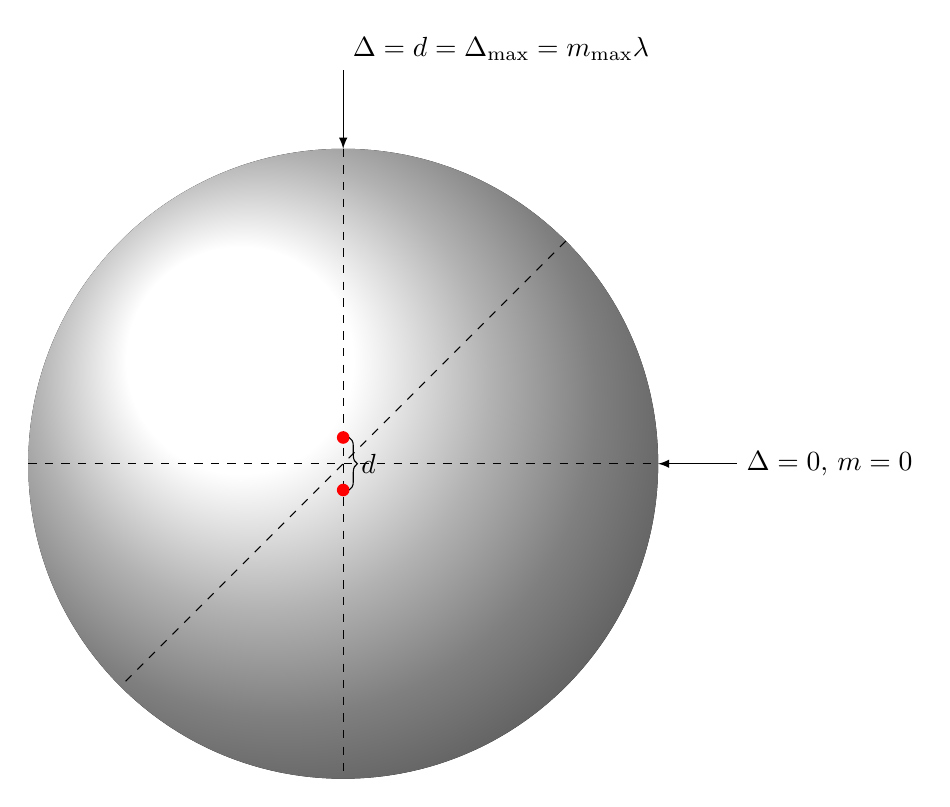
\begin{tikzpicture}
  \def\R{4} % sphere radius
  \def\Elevation{20} % elevation angle
 

  \fill[ball color=white!10] (0,0) circle (\R); % 3D lighting effect

\foreach \i in {89,86,...,59} {
\DrawLatitudeCircle{\i}
\DrawLatitudeCircle{-\i}
}
\foreach \i in {-6,-3,...,6} {\DrawLatitudeCircle{\i}}
\draw[dashed] (0,\R) -- (0,-\R);
\draw[dashed] (-\R,0) --(\R,0);
\draw[dashed] (45:\R) -- (225:\R);
\fill[red] (0,\R/12) coordinate (S1) circle (0.08);
\fill[red] (0,-\R/12) coordinate (S2) circle (0.08);
		\draw[decorate,decoration={brace,amplitude=3pt, raise=0.5ex}] (S1) -- node[right=3pt] {$d$} (S2);

\draw[latex-] (90:\R) -- ++(90:1) node[above right] {$\Delta = d= \Delta_{\max} = m_{\max}\lambda$};
\draw[latex-] (0:\R) -- ++(0:1) node[right] {$\Delta = 0$, $m = 0$};
\end{tikzpicture}  
\caption{Інтерференційні картини при різних положеннях екрану
відносно двох точкових монохроматичності джерел}
\label{fig:IntPic}
\end{figure}

\section{Реальні схеми спостерження інтерференції}

Для отримання когерентних світлових хвиль застосовують спеціальні експериментальні методи. Ці методи можна розділити на два класи:
\begin{itemize}
	\item методи поділу хвильового фронту;
	\item методи поділу амплітуди.
\end{itemize}

Їх ідея полягає в тому, щоб використовувати випромінювання одних і тих самих атомів джерела.

В \emph{методі поділу хвильового фронту} інтерферують хвилі, що йдуть від різних ділянок хвильового фронту. На цьому методі побудовано класичні інтерференційні схеми: дзеркало Ллойда, біпрізма Френеля, білінзи, бідзеркала, дослід Юнга тощо \cite[\S  5, стор. 81]{Godzhaev}.

В \emph{методі поділу амплітуди} пучок ділиться на одній або декількох пропускаючих поверхнях, що частково відбивають світло. Амплітуда кожної з інтерферуючих хвиль меньша ніж амплітуда вихідної хвилі. Даний метод використовується для спостереження інтерференційної картини в тонких плівках, інтерферометрі Майкельсона, інтерферометрі Фабрі-Перо \cite[\S 6, стор. 85]{Godzhaev}.

Якщо джерело світла точкове, то в результаті застосування оптичної схеми будь-якого з методів розподілу (хвильового фронту або амплітуди) виникнуть два точкових зображення джерела, які стануть новими когерентними джерелами. Випромінювання від цих нових джерел буде поширюватися, взагалі кажучи, не у всіх напрямках (це залежить від
оптичної схеми). Інтерференція буде спостерігатися в області накладення
світлових пучків від обох джерел (в області інтерференції) при будь-якому
розташуванні екрана. У цьому випадку говорять, що інтерференційна картина
не локалізована. Як вже зазначалося вище, вигляд інтерференційної картини
залежить від взаємного розташування лінії, що з'єднує джерела, і
площині екрану. Якщо лінія паралельна площині екрану (схема Юнга), то
спостерігаються смуги. Якщо лінія перпендикулярна площині екрану, то
спостерігається система кілець.